\documentclass[11pt,oneside]{amsart}
\usepackage{alttpreamble}
% \usepackage{tocloft}
% \renewcommand{\cftsecleader}{\cftdotfill{\cftdotsep}}
\newcommand{\minus}{\scalebox{0.8}{$-$}}
\newcommand{\plus}{\scalebox{0.6}{$+$}}
\begin{document}
\author{Maya Basu}
\author{Ethan Clayton}
\author{Fredrick Mooers}

\address{University of California, Berkeley}
\email{mab@berkeley.edu}

\address{University of Illinois, Urbana-Champaign}
\email{ewc3@illinois.edu}

\address{Virginia Tech}
\email{mooersfl24@vt.edu}

\title{Persistent Legendrian contact homology in $\R^3$}



\subjclass{53D42; 53D10, 57K10; 55N31}
\keywords{Legendrian contact homology, Legendrian knot, Persistent Homology}

\maketitle

\tableofcontents
\newpage

\section{Flooding the Knot}

Consider a Legendrian Knot in the Lagrangian projection. The knot diagram is sectioned into \textit{regions}, enclosed (signed) areas, with total signed area zero. Given a region in the knot diagram, pick a starting point on the boundary of the region and travel counterclockwise around the boundary, marking each transverse double point (corner in the boundary) passed with a positive or negative sign depending on the Reeb sign. By Stokes' theorem, the signed sum of the Reeb heights of these double points must be strictly greater than zero.

\begin{definition}[Reeb Inequalities]
\label{def:ReebIneq}
The collection of inequalities (one for each region) obtained in the manner above is called the \textit{Reeb inequalities}.
\end{definition}

\begin{example}[Trefoil Area]
\TODO: Add knot diagram.
    
\end{example}
\subsection{Algebraic Description}
Consider the set of all inequalities obtained by creating a chart for the knot. Follow the following procedure:
\begin{algorithm}
\label{alg:AlgFlood}
    \begin{enumerate} 
        \item Set $n = 1$
        \item Considering the (finite) collection of inequalities in the knot chart, find the generators $g_1 \cdots g_k$ which are only listed as positive terms in every inequality.
        \item Assign generators $g_1 \cdots g_k$ to tier $n$.
        \item Delete every inequality in the knot chart which contains at least one copy of any of the generators $g_1 \cdots g_k$.
        \item Increment $n$ by $1$, and repeat steps $2$ through $5$, until the knot chart is empty, meaning there are no remaining inequalities
        \item Any remaining generators not yet assigned to a tier are placed in the "extras" tier
    \end{enumerate}
\end{algorithm}

\subsection{Geometric Description}

Consider the set of all loops which are described by an inequality in the knot diagram. Label each corner of an intersection as $+$ or $-$ as whether traversing the intersection counterclockwise goes from an over-strand to an under-strand ($+$) or from an under-strand to an over-strand ($-$)

\begin{algorithm}
\label{alg:GeomFlood}
    \begin{enumerate} 
        \item Set $n = 1$
        \item Consider every generator $g_1 \cdots g_k$ where every negative corner of the crossing is in a shaded region. 
        \item Assign generators $g_1 \cdots g_k$ to tier $n$.
        \item Shade in ("flood") each region which is an area loop including these generators
        \item Increment $n$ by $1$, and start from step $2$, until the knot is completely flooded.
        \item The remaining generators are placed in the "extras" tier.
    \end{enumerate}
\end{algorithm}


Figure \ref{fig:Flood} shows the geometric flooding algorithm preformed on one of the Chekanov pairs, $m(5_2)$. The color brightness represent at what point in the algorithm the area loop was removed, with lighter coloring meaning being removed later.


\begin{figure}[htbp]
  \label{fig:Flood}
  \centering
  \includesvg{Pictures/CE2.svg}
  \caption{Flooding Algorithm on $m(5_2)$.}
\end{figure}


% \subsection{Observations}
% 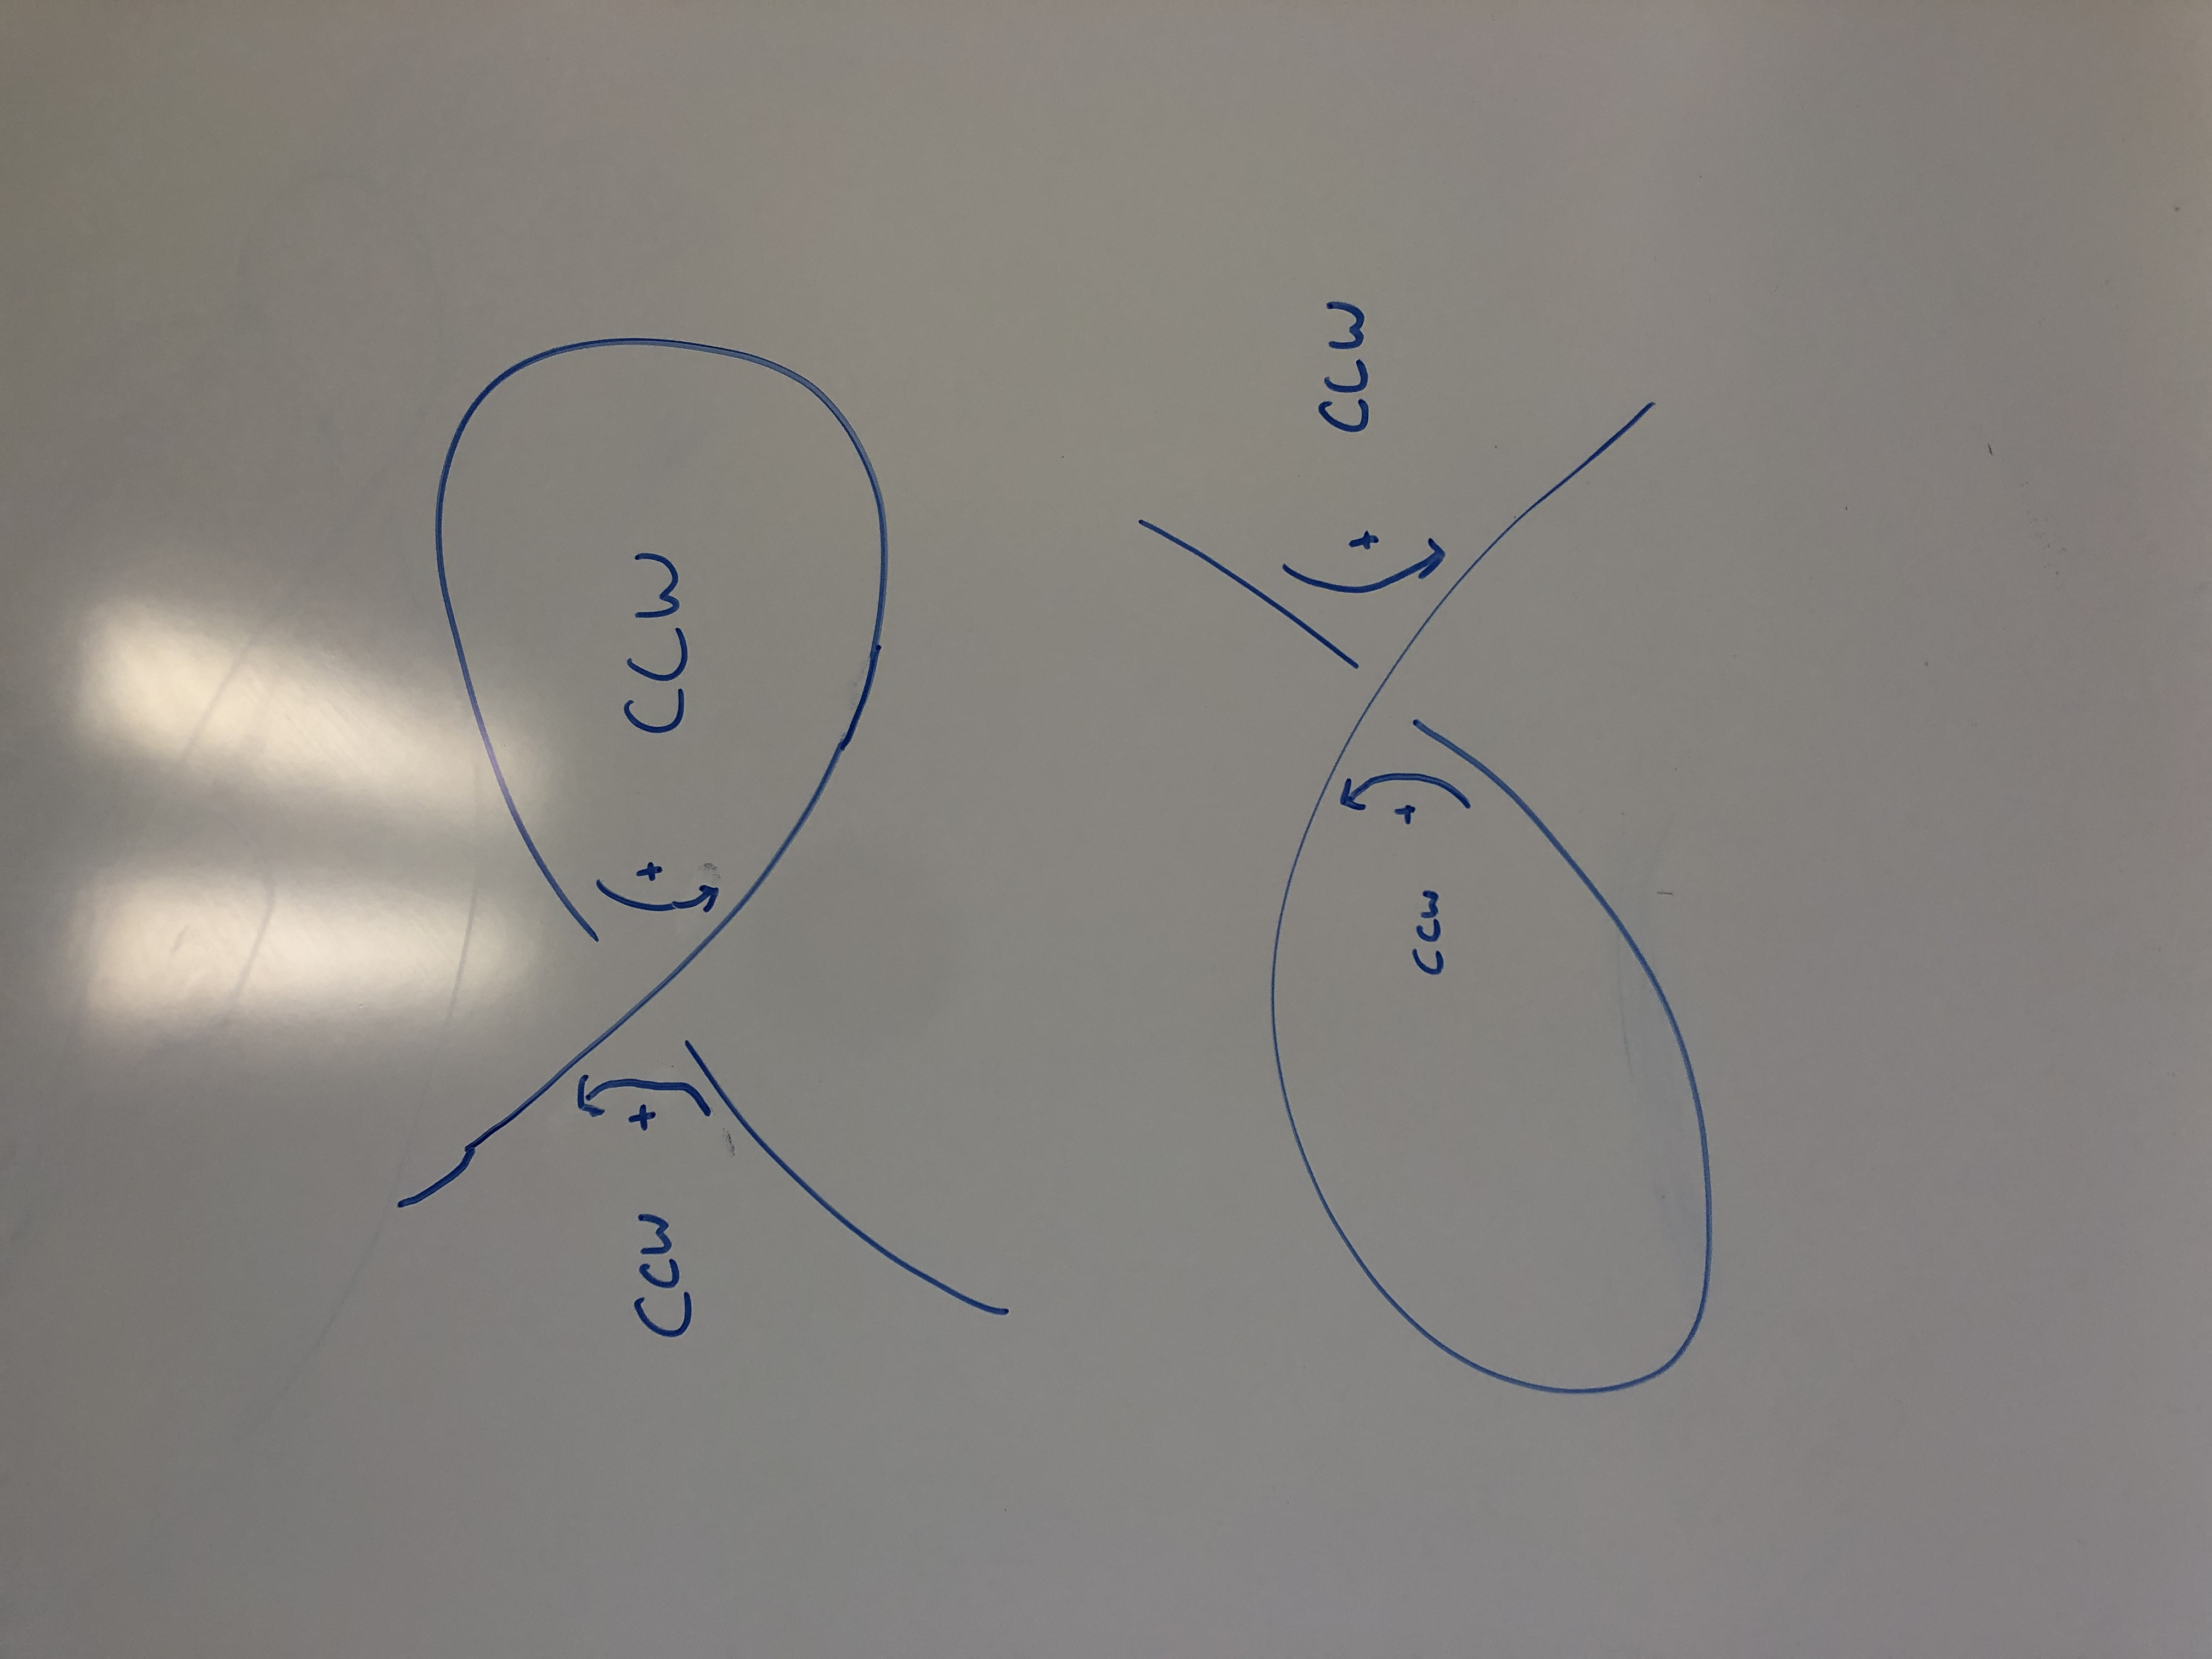
\includegraphics[width=4in,angle=-90]{Pictures/Exterior Loops.JPG}
% 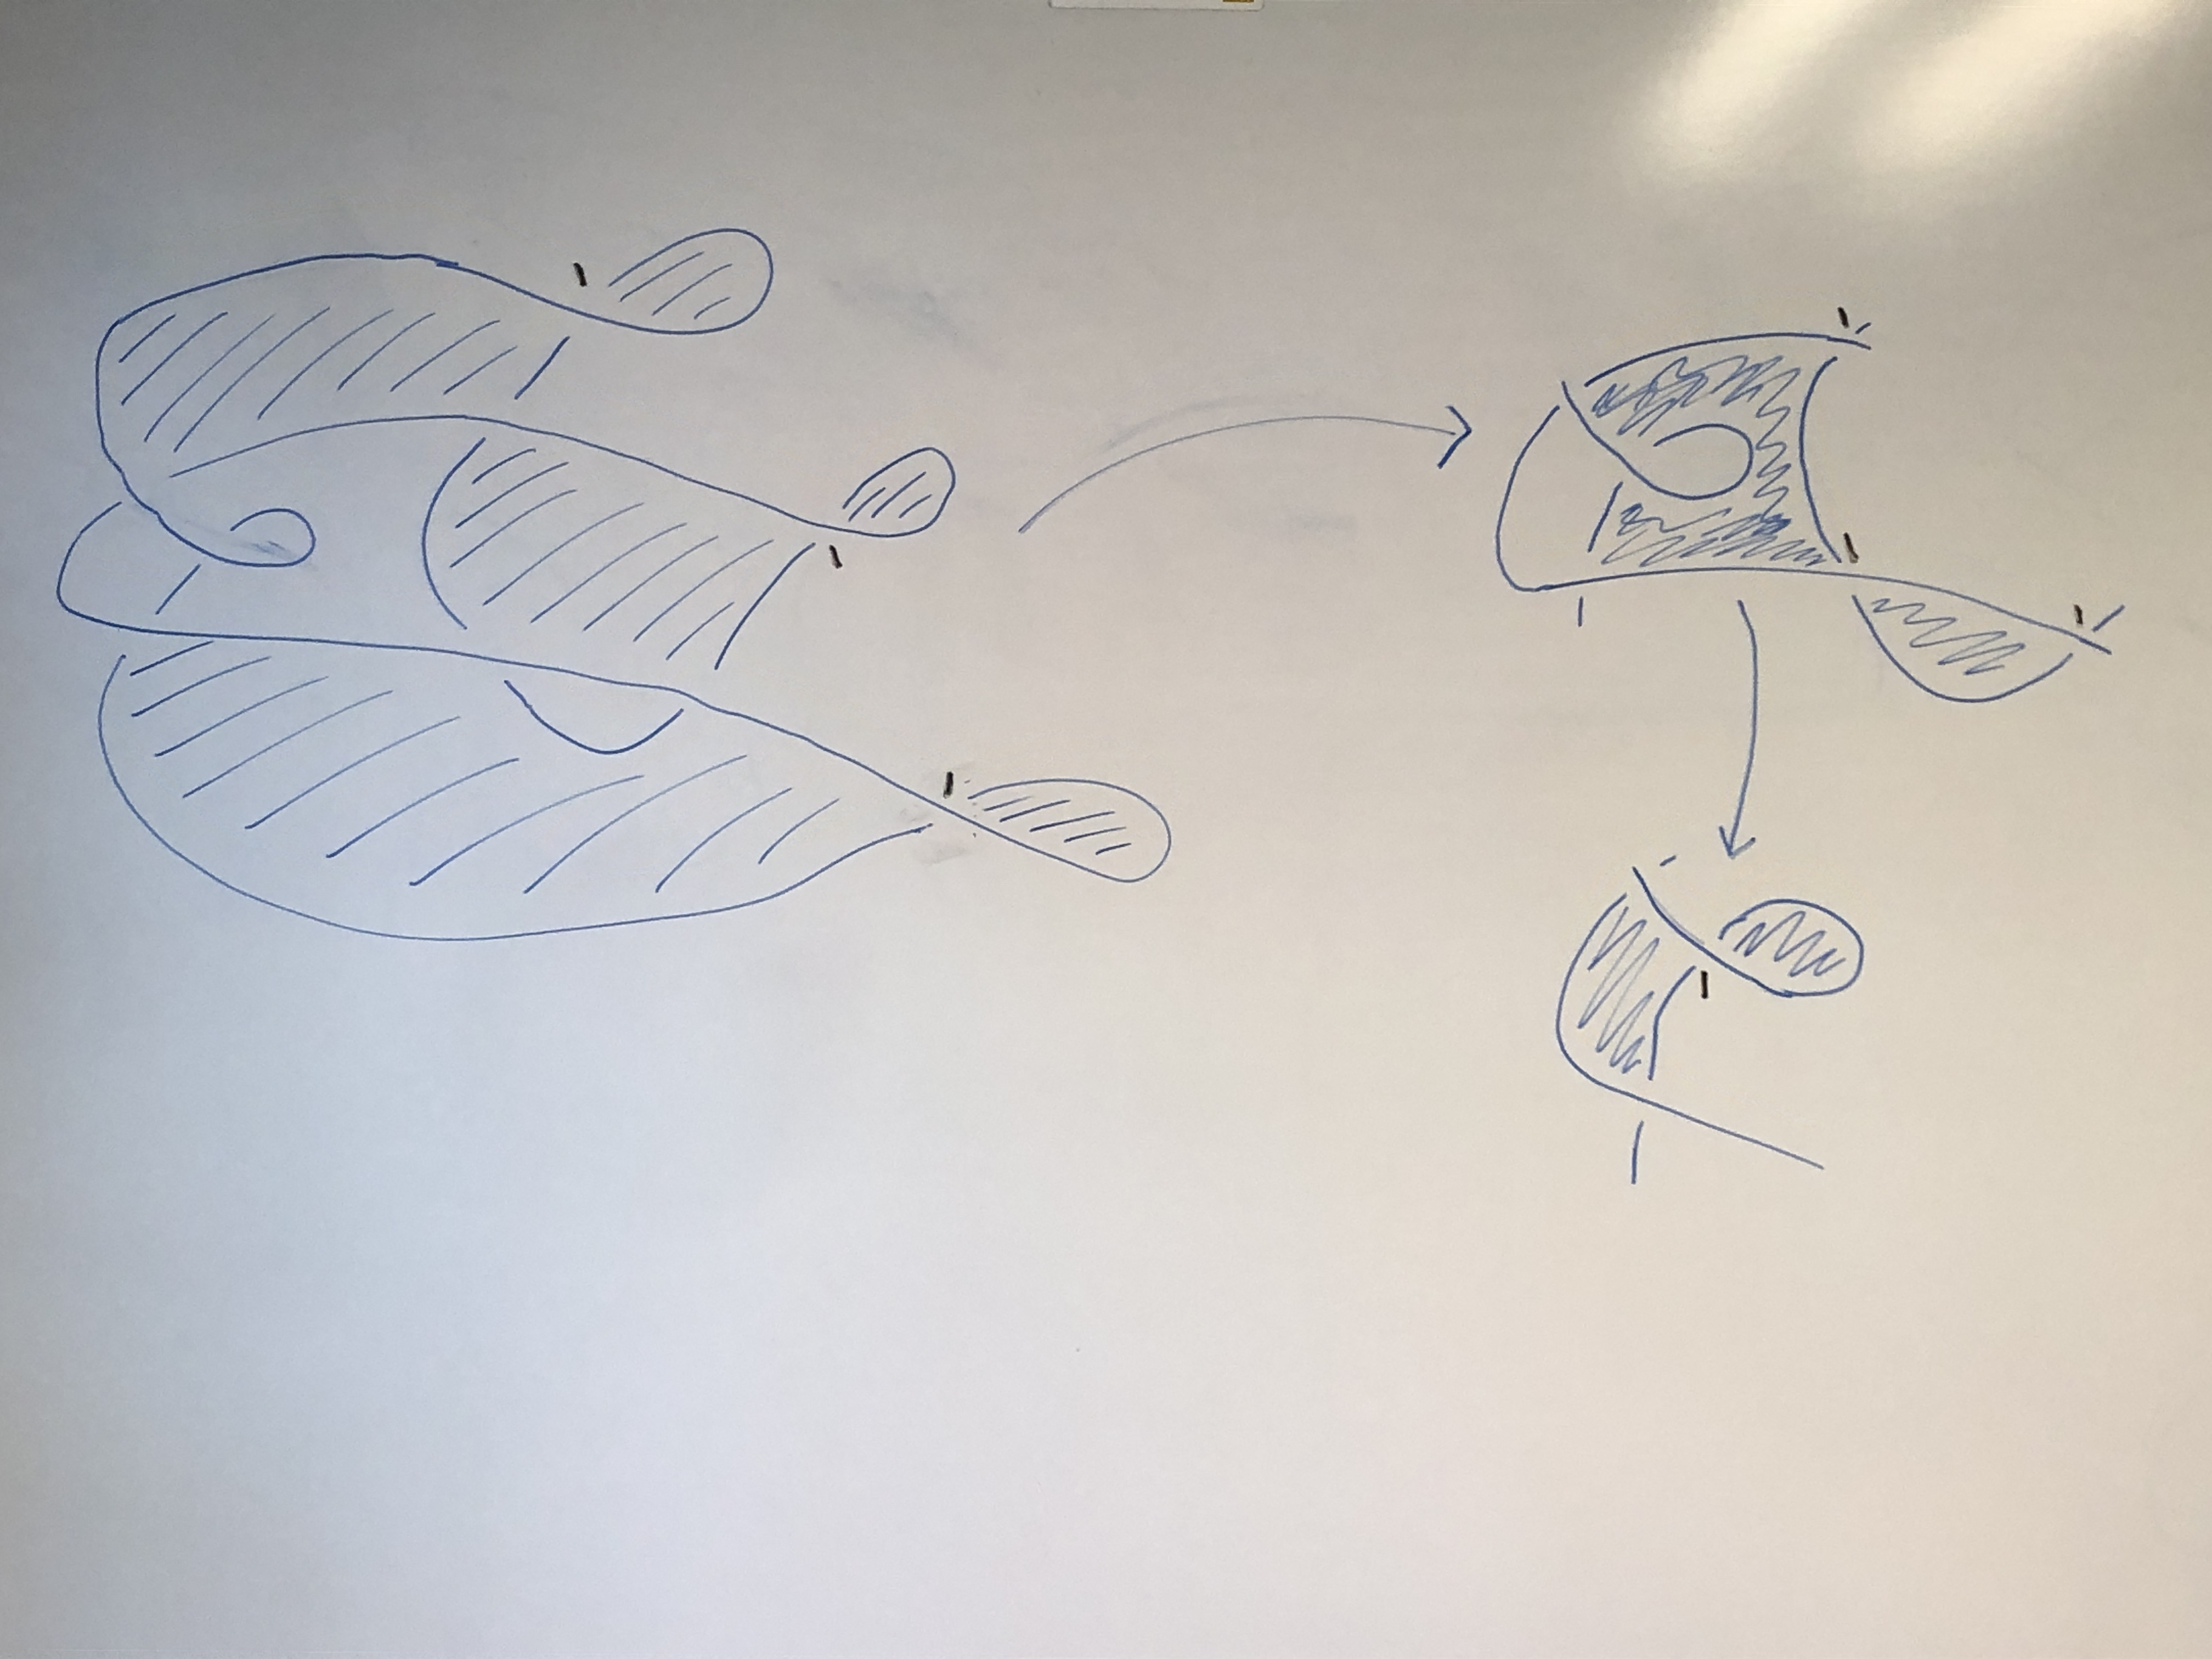
\includegraphics[width=4in]{Pictures/Visualization of Algorithm.JPG}
% In this manner, continue through to the nth free generators, obtaining n classes of freedom, "the extras" are class n, which are never only positive in the remaining equations
% \[f^{1}_1 \cdots f^{1}_{k_1} > f^{2}_1 \cdots f^{2}_{k_2}> \cdots > f^{n-1}_1 \cdots f^{n-1}_{k_{n-1}} > k_n \text{ extras }\]


\subsection{Assigning Heights}

This algorithm gives a set of valid relations on the Reeb heights from the height inequalities, but certainly not the only. Given the tiers $A_n=\{a^{(n)}_i\}_i$ where the $a^{(n)}_i$ are Reeb chords. We can assign any heights that satisfies $h(a^{(n)}_i)>h(a^{(m)}_i)$ when $n\leq m$.
\begin{theorem}
    Maybe we should prove that.
\end{theorem}
\begin{proof}
    
\end{proof}



\subsection{Proof of algorithm in a special case}


\begin{theorem}
    If a Legendrian Knot is in plat position and Ng's algorithm is applied, then for the resulting Lagrangian projection, our algorithm will always terminate.
\end{theorem}

\begin{proof}
    There are a finite number of total intersection within the knot. Therefore, if we can show that in each cycle of the algorithm, at least one intersection is placed into a tier, then the total number of remaining intersection is strictly decreasing and the algorithm must terminate.

    For any tier in the algorithm, consider the rightmost remaining intersection. It has two negative signs, above and below. By the nature of plat position, these negative signs are in a loop with a positive sign at an intersection to the right. Since by assumption those intersections are already cleared, the loops above and blow are filled in. Now there are two cases, either the intersection has only positive crossings remaining, or it is empty on the right and is thus an extra.

    If the intersection has only positive crossings remaining it is in the next tier and we are done. If the intersection is an extra then we must move to the next rightmost remaining intersection. Again this intersection has two negative signs, above and below which must have loops with positives to the right. The only intersections to the right are ones already covered or the extra we from the previous step. It a negative crossing has an extra to the right then it must be on an exterior loop since the extra is empty on the left. Otherwise, the negative crossing has an already covered positive to the right and is thus covered. In either case the new intersection has both negative crossings eliminated. Thus we are in the same position as before and the crossing is either in the next tier or an extra. If it is an extra we repeat this process until we find a non-extra or we have gone through all intersection.

    If we find an non-extra then it is placed in the next tier. Therefore each tier in the algorithm reduces the total number of remaining loops by one, and the algorithm must terminate. If there are no non-extras then all remaining intersections are places in the extras category and the algorithm also terminates. 
\end{proof}

\begin{figure}[htbp]
  \label{fig:PlatProof}
  \centering
  \includesvg{Pictures/proof1.svg}
  \caption{In plat, we trust.}
\end{figure}

\begin{remark}
All extras are "super" contractible (these are generators which are never responsible for shading a loop - therefore they can \textbf{all} be set equal to zero \textbf{simultaneously}.

Not all contractible chords are super contractible - some chords may go to zero iff one of the other positive generators in their loop increases by some finite amount. 

If there are no extras (super contractible chords) than the last class are contractible, as the lack of extras implies the last set of equations to be crossed out contains no negatives. 

Contractible chords can be in classes other than the last/extras class. For example, a stabilization introduced a contractible chord in the second class.

When attempting to 'swap' the heights of generators we observed that an element from a lower tier, can not be made greater than all of the heights of the tier above simultaneously, only some of them.

When doing Reidemeister move one in the front projection, we found that it added a single finite line to the bar-code in $H_0$, with a single (one element) generator. We hypothesize that this is always true, and so when finding an equivalence relation for bar-codes, we can 'mod out' theses types of lines. We will do more examples and test the other two Reidemeister moves.    
\end{remark}


\section{Algebraic description of contractability}
{\color{red} \textsc{This section needs to be modified.}}
\begin{definition}[Contractible]
    A Reeb chord $a$ is contractible if the Reeb inequalities still hold when the height of $a$ is set to $0$ ignoring any $0>0$ obstructions.
\end{definition}

A contractible crossing is a generator $a_i$ in the area inequalities where for each inequality that $a_i$ appears as positive, there are no other negative terms, or if there is one or more negative terms, there is at least one other positive term. {\color{red} \textsc{This is no longer true. See $m(5_2)$ for the simplest example.}}

This is a necessary condition for contractibility, but not sufficient, as if we take the "actual" definition of contractibility to be a legandrian isotopy up to the endpoint where the height goes to zero. This can not happen if the above requirement is not satisfied, however, the above requirement does not automatically guarantee the existence of such a legendrian isotopy. 

\begin{lemma}
    \label{lem:extradesc}
    For a Legendrian $\L$ with $F(\L)$ in plat position, the extras of the flooding algorithm are crossings that eventually look like ``pinch crossings''
\end{lemma}
\begin{proof}
    Algebraic v. Geometric picture clear \TODO
\end{proof}

\begin{definition}
    \label{def:doubleshade}
    A crossing $a$ in $F(\L)$, that isn't an extra of the flooding algorithm, \textit{double shades at tier $n$} if every inequality at the $n$th step of the flooding diagram that $a$ appears in contains another Reeb height with positive sign. If $a$ double shades at all tiers, we say $a$ double shades.
\end{definition}

% \begin{lemma}
%     For $F(\L)$ in plat position, a crossing double shades or is an extra at tier $n$ for some $n$ if and only if it double shades or is an extra at all tiers.
% \end{lemma}

\begin{lemma}
    \label{lem:doubleshadecrit}
        For $F(\L)$ in plat position, a crossing double shades at tier $1$ if and only if it double shades at all tiers.
\end{lemma}
\begin{proof}
    The forward direction is trivial. For the backwards direction, not that if $a$ double shades at tier $1$, then it double shades at least until it's removed at tier $n$. If there is a region to the left of $a$, then we're done. If there isn't a region to the left of $a$ then note that the crossing on the other side of the region to the right of $a$ (when a left crossing exists a right cusp or crossing to the right exists) also exists while $a$ is breathing. If this weren't the case, then $a$ would be negative in all Reeb inequalities at time $n$ and thus making it an extra. Hence, $a$ drowns with its right region flooding meaning $a$ double shades for all tiers.
\end{proof}

\begin{proposition}
    \label{prop:contractdesc}
    For $F(\L)$ in plat position, a Reeb chord corresponding to a right cusp or double point, $a$, is contractible if and only if $a$ double shades or is an extra or corresponds to a left loop in $\Pi(\L)$.
\end{proposition}

\begin{proof}
    ($\Rightarrow$) Assuming that $a$ doesn't double shade, we must show that $a$ is never removed by the flooding algorithm (i.e. $a$ is an extra) or is removed at the last step on the algorithm (i.e. $a$ corresponds to a left loop in $\Pi(\L)$). Since $a$ is contractible, the region to the left, if it exists, corresponds to an inequality that has no negatives. Such an inequality can exist precisely when $a$ corresponds to a left loop in $\Pi(\L)$. If a left region doesn't exist, then since $a$ doesn't double shade, it follows that a right region at a certain step in the algorithm floods before the algorithm terminates, and hence $a$ is an extra.

    ($\Leftarrow$) Clearish?
\end{proof}

\begin{corollary}
    \label{cor:contractenum}
    The flooding algorithm enumerates contractible Reeb chords for a legendrian $\L$ with $F(\L)$ in plat position.
\end{corollary}


\subsection{Stabilization}
Adding a stabilization with generator $a_j$ creates a contractible reed chord, because we add two things to the area inequalities: $a_j>0$ and we add a positive $a_j$ to one other area inequality. Because we previously had a valid knot, there must have been at least one other positive in this latter equation, so the added $a_j$ satisfies the necessary conditions of contractibility. 



\section{Bar Codes and Suffering}

\subsection{Stabilization}

    Any Legendrian Isotopy of knots induces a stable time Isomorphism at the level of DGA's.  We planned to examine the effects that stabilizations and tame isomorphisms have on the persistence module barcode, to understand which parts are homologically significant. 
    
    We found that a grading $k$-stabilization, adds a single finite bar to $H_{k-1}$ which is generated by a single element. On the level of DGA's, a grading $k$-stabilizations adds two generators $e_k$ and $e_{k-1}$. $e_k$ has grading $k$ and $e_{k-1}$ has grading $k-1$, and their differentials are given by $\d (e_k) = 1 + e_{k-1}$ and $\d e_{k-1} = 0$. After linearizing this must give linear differentials $\d^\epsilon (e_k) = e_{k-1}$ and $\d^\epsilon e_{k-1} = 0$. 

    The generator $e_{k-1}$ causes a finite bar to be born at time $h(e_{k-1})$. and since $\d^\epsilon (e_k) = e_{k-1}$, this bar dies at time $h(e_k)$. This bar has generator $e_{k-1}$. This Stabilization also has no effect on any other differentials, so it does not alter any other bars, finite or otherwise.

\subsection{Tame Isomorphisms are too General}

    A tame isomorphism can change the number of generators for any bar. For example, if a bar is generated by $a_1 + \cdots a_n$, then we can have a tame isomorphism that sends $a_1$ to $a_1 + a_2 + \cdots a_n$, and all other generators to themselves. After this tame isomorphism, the bar will be generated by $a_1$.

    Furthermore, any finite bar can be removed by a tame isomorphism and destabilization (\TODO prove). This means that Reidemeister moves will be important to our argument.

\subsection{$H$-contractibles are inessential}
    \begin{definition}
        For a persistence module barcode we call a finite bar $H$-contractible, if there is a valid assignment of heights to Reeb chords such that for any $\varepsilon > 0$
        \begin{enumerate}
            \item For any Reeb Chord $a_i$, the height $h(a_i) \geq 1$
            \item the length of the bar $l < \varepsilon$
        \end{enumerate}
    \end{definition}

    We claim that any $H$-contractible bar is homologically inessential, and that any bar which is not $H$-contractible is homologically essential.

$H$-contractible bars are by definition invariant under planar isotopy, since planar isotopy only corresponds to a reassignment of Reeb heights.

Observation: When doing a Reidemeister move 2 onto the trefoil, we added a new $H$-contractible bar. We also altered the existing finite bar. However it remained not $H$-contractible, which is a good sign. That bar is born at the max of $a_3$ and $a_5$, and is killed either by $a_2$ of $a_1$ and $b_2$. However, we have that $a_2$ must be larger than $a_3 + a_4 + a_5$ and $a_1$ must be larger than $b_1 + a_3 $ and $b_2$ must be larger than $a_4 + a_5$. (+ > max).

Problem: We found that if you do a Front projection Reidemeister move 1, and then a second Front projection Reidemeister move 1 on top of the previous move, the previous $H$-contractible bar that was created by the first move is made not $H$-contractible by the second move. This is because the differential is altered. This gives us a new definition

\begin{definition}
    A \textit{valid height assignment (or valid planar isotopy)} is a assignment of Reeb heights satisfying the inequalities and the heights of all non-contractible are kept greater than 1.
\end{definition}
\begin{definition}
    For a persistence module barcode we call a finite bar $H$-contractible, for any $\varepsilon > 0$, there is a valid assignment of heights to Reeb chords such that the length of the bar $\ell < \varepsilon$.
\end{definition}


\subsection{A new equivalence relation?}

We believe that we can get all information about $H$-contractible bars strictly from the differential. The only restriction we have on the $H$-contractible bars is if we have an area loop where there is one positive and a set of negatives such that at least one of the negatives which is not in the canceled cycle is not contractible. However this gives an area loop which has one positive and the rest negative, which is precisely the definition of a disk. If instead we got this inequality from a sum of area loops this would still form a valid disk since it has to cancel out terms properly.

\subsubsection{Planar Isotopy}

Since planar isotopy is equivalent to a reassignment of Reeb Heights, either a planar isotopy will give a set of Reeb heights that is valid for our definition of $H$-contractible, or it will give a set of Reeb Heights which is valid. In either case the set of all valid Reeb heights that can be achieved by planar isotopy has not changed, and the DGA has not changed, so the $H$-contractible and non-$H$-contractible bars will not change.

\subsubsection{Move I}
{\color{red} \textsc{Assumption (Big Assu): There is a valid planar isotopy making $h(a)\rightarrow h(b)+h(c)$}.} Assume $\alpha$ is not $H$-contractible. Then there exists $\varepsilon>0$ such that for all valid height assignments, $\ell(\alpha)\geq \varepsilon$. But then this means that $\ell(\alpha)\geq \varepsilon$ even in the case when $h(a)\rightarrow h(b)+h(c)$, if we make $h(a)-h(b)-h(c)$ small enough then we can add $h(b)+h(c)-h(a)$ to any previous height inequalities and still have a proper inequality meaning we can keep the same Reeb heights before and after Move I is performed. Hence, since the DGA doesn't change we know that (we don't necessarily know that we can get all possible planar isotopies now (immediately)). However, if we can show that what not being $H$-contractible means to the differential, then that's enough because the differential is preserved by planar isotopy, then we're so boujee (we hope).




\subsubsection{Move II}
{\color{red} \textsc{Assumption (Big Assu): There is a valid planar isotopy making $h(a)\rightarrow h(b)+h(c)$}.}

As described by both Chekanov and Etnyre, Ng, and Sabloff, at the level of DGA's this Reidemeister move corresponds to a tame isomorphism, which sends $a_3 \rightarrow a_3 + a_1a_2$. 

Assume $\alpha$ is a finite bar which is not $H$-contractible. Then $\epsilon>0$ such that for all valid height assignments, $\ell(\alpha) < \varepsilon$. We then look at three cases, one where $\alpha$ is generated by $a_3$, one where $\alpha$ is killed by $a_3$, and one where $\alpha$ has no $a_3$ term.

If 


\subsubsection{Move III}

S


\section{A Fresh Start}

\subsection{Area-Related Inquiries}

\begin{lemma}[Chekanov]
    Given an area loop $\gamma_i$ with bounding area $f_i$ and height equation $\sum_j E_{ij}h_j=f_i$, then $\sum_j E_{ij}|a_j|=2-(\# \text{ of positive corners in } \gamma_i)$.
\end{lemma}

\begin{lemma}[Us]
    Let $\Pi(\Lambda_-)$ and $\Pi(\Lambda_+)$ be related by triple point move II. Then 
        \[\Area(\Lambda_+)-\Area(\Lambda_-)=\left(-\delta_1 + \delta_2 -\delta_3 + \delta_4 - \delta_5 +\delta_6\right)(b+c-a)\]
    where $b+c-a$ is the area of the triangle considered in the triple point move and $\delta_i$ is 1 precisely when the knot contains (bounds) the $i$-th region seen in the figure below (\TODO).
\end{lemma}
In particular, the unsigned area of the knot can only change by a discrete shift by $m(b+c-a)$ for $m\in\{0,\pm1,\pm2,\pm3\}$ and if $b+c-a\in \Z$, then the unsigned area changes by a discrete amount.\footnote{Is $m=\pm3$ possible?}

\begin{lemma}[Us]
    Let $\Pi(\Lambda_-)$ and $\Pi(\Lambda_+)$ be related by double point move. Then 
        \[\Area(\Lambda_+)-\Area(\Lambda_-)=\left(\delta_1 + \delta_2 -2\right)(a-b)\]
    where $b+c-a$ is the area of the triangle considered in the triple point move and $\delta_i$ is 1 precisely when the knot contains (bounds) the $i$-th region seen in the figure below (\TODO).
\end{lemma}


\subsection{Experiments in Preserving Area with the Platypus Knot}

Our method of experimentation is as follows. First we consider the Platypus Knot (plat position $4, 3, 2, 3, 2, 4$) and use Integer Programming (mathematica) to find the minimum area under the constrants that the heights are integral and positive, and that the minimum area of each area patch is $1$. This gives us that the heights of the generators are 
\[h(a_1) = 1\]
\[h(a_2) = 2\]
\[h(a_3) = 1\]
\[h(a_4) = 1\]
\[h(a_5) = 1\]
\[h(a_6) = 3\]
\[h(a_7) = 3\]
\[h(a_8) = 4\]
\[h(a_9) = 5\]
which, considering that the area equation is $2a_9 + 2a_8+2a_7 - a_5 - a_6-a_3+a_2 - a_1$ gives us a minimum area of $20$. Additionally, mathematica gives that this is the only such assignment of heights such that the total unsigned area is $20$. 


Now, we attempt to preform Reidemister move $3$ on the Platypus Knot to get $4,2,3,2,2,4$. If we restrict the area to still be $20$ and require that areas be greater than $1$ and reeb heights remain integral there are no solutions (not particularly supprising). If instead we allow reeb heights to be in the reals, then we can get a solution (we set the minimum reeb height to be $10ˆ{-1}$): 

\[h(a_1) = 0.1\]
\[h(a_2) = 2.4\]
\[h(a_3) = 1.1\]
\[h(a_4) = 0.1\]
\[h(a_5) = 0.1\]
\[h(a_6) = 2.1\]
\[h(a_7) = 3.6\]
\[h(a_8) = 4.4\]
\[h(a_9) = 3.2\]


Doing persistent homology on both of these knots shows that several of our most imediate hypothesis are false. First, the total length of all finite bars is not preserved. Nor is any imediatly obvious ratio of lengths of these bars. 




Suppose that we consider how the heights change if the total area is fixed at $20$, area loops except the triangle are restricted to greater than $1$, and the minimum reeb height is restricted above a small value (I picked $0.001$). The question is, as we decrease the triangle area, is it possible to find a solution at every step of the way? Meaning can we preform move $3$ with area conserved along the way as the triangle is isotoped to be smaller than the surrounding areas?

Trying the triangle area set to $1,0.5,0.1$, then $0.1,0.5,1$ after the move, here is the plot of how the reeb chord heights change (here $y_i$ is the height of $a_i$).

\begin{figure}[htbp]


  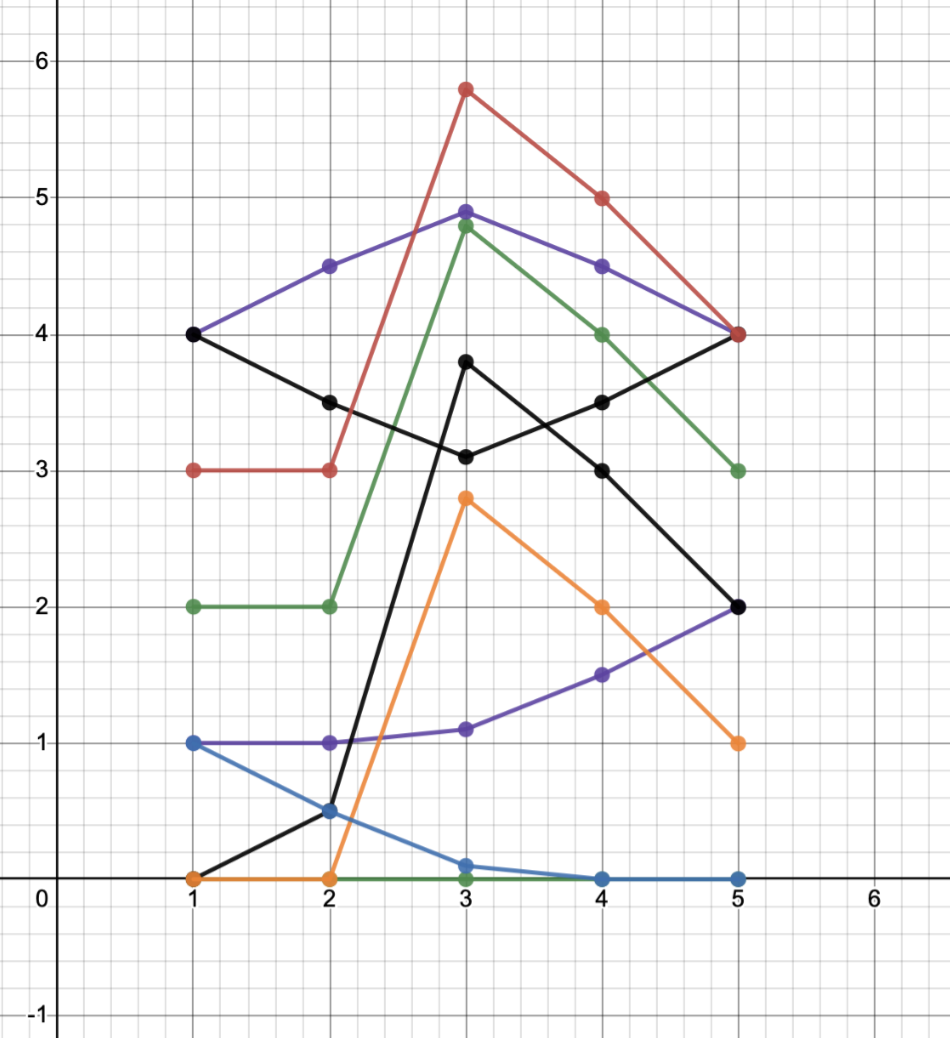
\includegraphics[width = 3in]{Pictures/heightschangegraph.png}
   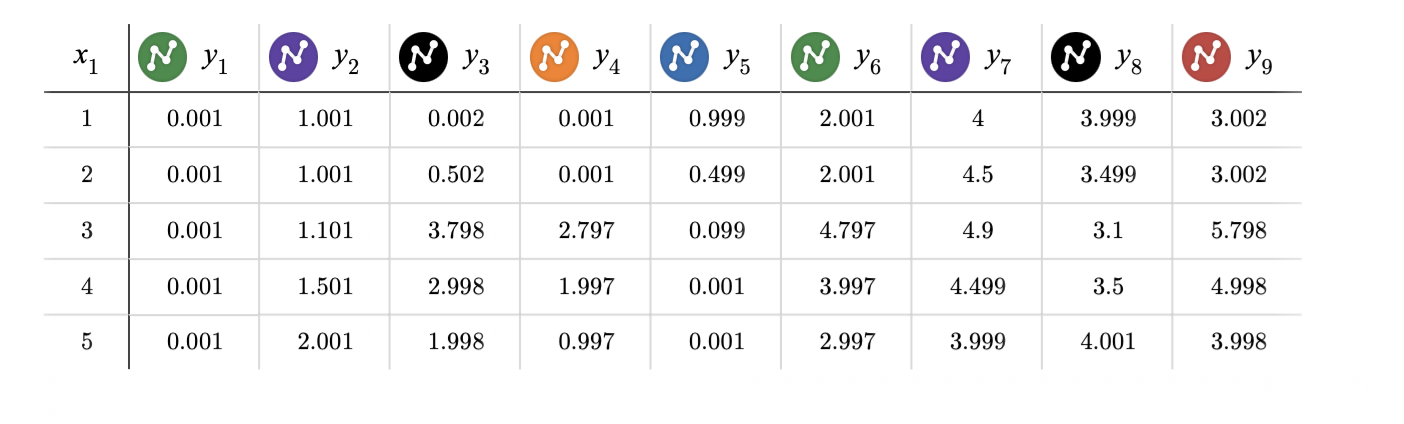
\includegraphics[width = 3in]{General-Information/Pictures/heightchangetable.png}
  \caption{Reeb Heights as Reidemister 3 is preformed under area constrained to 20}
  
\end{figure}

There is a strange discontinuity in the reeb heights, however this might simply be an artifact of the fact that there may be many height assignments that give us the minimum area of $20$. Notably though, there does appear to be solutions which satisfy all of the requirements, namely that all other areas are greater than $1$ and the total area is $20$.










\subsection{Net Unsigned Area After Reidemeister move}

After Reidemeister move $2$, the net change unsigned area is (assuming no other Reeb heights change in the process)

\[\Delta A = (\delta_1 + \delta_2) \cdot (a - b) + b - a + \delta_{3}ˆ{\plus} (R_{3}ˆ{\plus} + b)+ \delta_{3}ˆ{\minus}(R_{3}ˆ{\minus} - a) - \delta_{3}ˆ{\plus}\delta_{3}ˆ{\minus}(R_3)\]

There are two distinct Reidemeister move 3's possible in the Lagrangian projection. Assuming that no Reeb heights change in the process we can again calculate the change in the unsigned area.

$\Delta A = (a-b-c)(-\delta_1+\delta_2-\delta_3+\delta_4-\delta_5+\delta_6)$ and
$\Delta A = (b+c-a)(-\delta_1+\delta_2-\delta_3+\delta_4-\delta_5+\delta_6)$


\section{$m_2$ product}
Goal: $\exists A_\infty$ products. Today we'll see one product structure, $m_2$. Setup: Let $\AlgL$ be the Chekanov-Eliashberg DGA of $\L$, with $\Z_2$ coefficients with $r(\L)=0$. Fix a single augmentation $\epsilon$. Let $A=\Z_2\{ a_1,\cdots,a_n\}$. As an algebra $\AlgL^\epsilon=\bigoplus_{i=0}^\infty A^{\otimes i}$. Notation: Use subscripts within parenthesis to denote word length. Use augmentation to get $\Phi^\epsilon:\AlgL^\epsilon \rightarrow \AlgL^\epsilon$ and $\d^\epsilon = \Phi^\epsilon \circ \d_\L \circ \Phi^{\epsilon}$. Consider the right handed trefoil with $|a_1|=|a_2|=1$ and $\epsilon(a_3)=1$. Then
    \[\d^\epsilon(a_1)=\underbrace{a_3+a_5}_{\d^\epsilon_{(1)}(a_1)}+\underbrace{a_5a_4}_{\d^\epsilon_{(2)}(a_1)}+\underbrace{a_5a_4a_3}_{\d^\epsilon_{(3)}(a_1)}\]
and
    \[\d^\epsilon(a_2)=\underbrace{a_3+a_5}_{\d^\epsilon_{(1)}(a_2)}+\underbrace{a_4a_5}_{\d^\epsilon_{(2)}(a_2)}+\underbrace{a_3a_4a_5}_{\d^\epsilon_{(3)}(a_2)}.\]
More generally, we have
    \[\d^\epsilon=\sum_{j=1}^\infty \d_{(j)}^\epsilon.\]
We have $\d{(2)}^\epsilon=0$ for anything of grading $0$ in the trefoil above.

Note that $\d_{(2)}^\epsilon:\AlgL^\epsilon \rightarrow A^{\otimes 2}$ and it restricts to linear transformation $\partial_{(2)}^\epsilon:A\rightarrow A^{\otimes 2}$.

\begin{definition}
    Let $m_2:(A^{\otimes 2})^*\rightarrow A^*$ be the formal adjoint of $\partial_{(2)}^\epsilon$. Since $A$ is finite dimensional, we can identify $A$ with it's dual. So we get a map $m_2:A\otimes A\rightarrow A$.
\end{definition}

We have $m_2(a_5\otimes a_4)=a_1$ and $m_2(a_4\otimes a_5)=a_2$ in the trefoil example. It's a degree +1.

\begin{proposition}
    For each $\ell$, we have
        \[0=\sum_{i+j+k=\ell} m_{i+1+k}\circ(\mathbf{1}^{\otimes i}\otimes m_j  \otimes \mathbf{1}^{\otimes k}).\]
\end{proposition}

\subsection{An important example}
It was known originally that $\\LCH_k(\L)\cong \\LCH_k(\overline{\L})$ for any $\L$. For our knot we have $|t_i|=|t_i^x|=|t_i^y|=|t_i^z|=1$ and $|a_1|=|a_2|=0$ and $|b_1|=-|b_2|=2$ and $|c_1|=-|c_1|=1$ and $|x_i|=|y_i|=|z_i|=0$. The differential $\d$ exists. Unique augmentation: $\epsilon(x_i)=\epsilon(y_i)=\epsilon(z_i)=1$ and other generators  map to $0$.
We have
\begin{align*}
    \d^\epsilon a_1&=0\\
    \d^\epsilon a_2&=c_1b_2+y_1c_1b_2\\
    \d^\epsilon b_1&=a_1c_1+a_1y_1c_1\\
    \d^\epsilon b_2&=0\\
    \d^\epsilon c_1&=0\\
    \d^\epsilon c_2&=b_2a_1+b_2a_1y_1 \\
    \d^\epsilon t_1&={\color{green}x_1}+a_1a_2+b_1b_2+\mathcal{O}\\
    \d^\epsilon t_2&={\color{green}y_1}+a_2a_1+c_1c_2+ \mathcal{0}\\
    \d^\epsilon t_3&={\color{green}z_1}+b_2b_1+c_2c_1+\mathcal{O}\\
    \d^\epsilon t_0&={\color{green}x_4}+y_3+z_1+x_4y_3+y_3z_1+x_4z_1+\mathcal{O}\\
    \d^\epsilon t_i^x&={\color{green}x_i}+x_{i+1}+x_ix_{i+1}\\
    \d^\epsilon t_i^y&={\color{green}y_i}+y_{i+1}+y_i y_{i+1}\\
\end{align*}
and $\dim A=23$ with $\text{rank}(\d_{(1)}^\epsilon: A\rightarrow A)=8$ and $a_1,a_2,b_1,b_2,c_1,c_2,x_i,y_i,z_i\in \ker{\d_{(1)}^\epsilon}$. We also have
    \[t:=\sum t_i + \sum t_i^x + \sum t_i^y\in \ker \d_{(1)}^\epsilon\]
and $\im \d_{(1)}^\epsilon=\Z_2\{x_i,y_i,z_i\}\cong (\Z_2)^8$
with $\\LCH_{\ast}^\epsilon=\Z_2\langle[a_i],[b_i],[c_i],[t]\rangle$.
We then have
    \begin{align*}
        m_2(c_1\otimes b_2)&=a_2\\
        m_2(a_1\otimes c_1)&=b_1\\
        m_2(b_2\otimes a_1)&=c_2\\
        m_2(a_1\otimes a_2)=m_2(b_1\otimes b_2)&=t_1\\
        m_2(a_2\otimes a_1)=m_2(c_1\otimes c_2)&=t_2\\
        m_2(b_2\otimes b_1)=m_2(c_2\otimes c_1)&=t_3\\
        m_2(x_i\otimes x_{i+1})&=t_i^x\\
        m_2(x_i\otimes x_{i+1})&=t_i^x\\
    \end{align*}
    \begin{align*}
        [c_1]\frown [b_2]&=[a_2]\\
        [a_1]\frown[c_1]&=[b_1]\\
        [b_2]\frown [a_1]&=[c_2]\\
        [a_1]\frown [a_2]=[b_1]\frown [b_2]&=[t]\\
        [a_2]\frown [a_1]=[c_1]\frown [c_2]&=[t]\\
        [b_2]\frown [b_1]=[c_2]\frown [c_1]&=[t]\\
    \end{align*}

When moving to the mirror $\overline{\L}$ we see the product structures are different.

\begin{question}
    How is $h(m_2(x\otimes y))$ related to $h(x)$ \& $h(y)$?
    Can tensor product on interval modules recover $m_2$, or at least the homology product? In the sense we can multiply bars as the tensor product of interval modules.
\end{question}



\section{Jul 10}

\begin{question}
    Can we use area on trigons and bigons. We need a deterministic way to assign heights and tell which are inessential.
\end{question}

Has 5 crossings but only 3 homologically essential generators that show up in it

\section{The only Legendrian knot is the trefoil}

\begin{theorem}

For any $\delta > 0$ and any Legendrian knot in the Lagrangian projection and any valid Lagrangian Reidemeister move for that knot there exists filtrations of the knot before and after the move such that the barcodes for the persistent homology of the knot before and after are $2\delta$-interleaved. Any augmentation of the knot prior to the Reidemeister move naturally gives an augmentation for the knot after the Reidemeister move, these are the augmentations that are used to create the barcode.

\end{theorem}

\begin{proof}

There are three Legendrian Reidemeister moves, we will call them Reidemeister move II, Reidemeister move IIIa, and Reidemeister move IIIb.

For Reidemeister move IIIa, take any Legendrian knot in the Lagrangian projection, assume there exists a triangle $abc$, with the area equation $a-b-c > 0$, such that a Reidemeister move IIIa can be performed. Then the Legendrian knots before and after the Reidemeister moves are Legendrian isotopic. Since Legendrian isotopy requires a continuous set of Legendrian knots, we must have for any $\delta > 0$, there exists planar isotopies before and after the move such that the triangle $abc$ has area less than $\delta/2$. Kalman describes how, the heights of the Reeb chords which make up the triangle can be made arbitrarily close to their original heights, i.e $< \delta/2$. Since the overall area of the triangle changes by less that $\delta/2$ and the individual heights for each Reeb chord in the triangle also change by less that $\delta/2$, the contributions that the Reeb chords in this triangle give to all other area loops changes by a maximum of $\delta$. Thus any other Reeb height must change by a maximum of $\delta$

Furthermore, under the Reidemeister move IIIa, DGA remains identical, meaning the set of augmentations are identical before and after the Reidemeister move. Since, all Reeb heights change by a maximum of $\delta$, the starting point and ending point of any bar in any augmentation can change by at most $\delta$ Therefore, for any augmentation, the barcodes generated by the knots before and after Reidemeister move IIIa are $2\delta$-interleaved 
    
\end{proof}

\begin{theorem}

For any Legendrian knot, given any augmentation, we can select a height assignment so there exists a bijection between the bars of the persistent homology and the bars in the persistent co-homology such that infinite bars are paired with infinite bars, and finite bars are paired with finite bars of the same length.

Furthermore the bijection maps finite bars in the k-th homology class to finite bars in the (k+1)-th co-homology class and infinite bars in the k-th homology class are mapped to infinite bars in the k-th co-homology class.

\end{theorem}

\begin{proof}
We have from {\color{red} paper} the short exact sequence
\begin{multline*}
    0 \rightarrow \Ext_{\mathbb{Z}_2[0,\infty)}(F^\bullet \LCH^\epsilon_{k-1},\mathbb{Z}_2[0,\infty))\rightarrow F^\bullet\LCH^k_\epsilon \\ \rightarrow \Hom_{\mathbb{Z}_2[0,\infty)}(F^\bullet\LCH^\epsilon_k,\mathbb{Z}_2[0,\infty)) \rightarrow 0
\end{multline*}
that (unnaturally) splits.
Hence, if $F^\bullet\LCH^\epsilon_k \cong \left[\bigoplus_{i_k} \mathbb{Z}_2[h_{i_k},\infty)\right]\oplus\left[\bigoplus_{j_k,m_k} \mathbb{Z}_2[h_{j_k}, h_{m_k})\right]$, then, for all $k$,
\[ F^\bullet\LCH^k_\epsilon \cong \left[\bigoplus_{i_k} \mathbb{Z}_2[-h_{i_k},\infty)\right]\oplus\left[\bigoplus_{j_{k-1},m_{k-1}} \mathbb{Z}_2[-h_{m_{k-1}}, -h_{j_{k-1}})\right]\]
Consider a finite bar in the homology which can be generated by a set of sums ${g_i}$, meaning that $\partial g_i = 0$ and killed by a set of sums ${k_j}$ meaning that $\partial k_j = g_i$ for some $i,j$.

Passing to the co homology, this means that we have that 

\end{proof}








\begin{proposition}
    It seems as though the essential finite bar in the Trefoil, it can be 'translated' to an infinite bar when examining persistent co-homology. Perhaps this could be a way of identifying essential bars
\end{proposition}







\begin{theorem}

The tame isomorphism induced by Reidemeister move IIIb commutes with the linearized differential

\end{theorem}


\begin{proof}

With the appropriate lableing of generators (see image), the tame isomorphism induced on the non linear DGA by Reidemeister move IIIb is the map $a \rightarrow a + bc$. Consider an arbitrary generator $x$ with non linear differential $\partial x$. This non linear differential consists of a sum of words of generators. We group these words into sums based on the number of times $a$ shows up. Noting that although the order of generators in a word matters in non linear differential, the order is made moot by the commutativity of the linear differential. As such, we may write

\[\partial x  = \sum (g_1^{0} \cdots g_{n_1}^{0}) + \sum (g_1^{1} \cdots g_{n_1}^{1})a + \sum (g_1^{2} \cdots g_{n_2}^{2})a^2 + \sum (g_1^{3} \cdots g_{n_3}^{3})a^3 \]

where the superscripts indicate which power of $a$ is present in a word that the generator is part of.

Now, let $\epsilon(a)$ be the augmentation of $a$. Then the augmented differential of $x$ is 

\[\partial^{\epsilon} x  = \sum ((g_1^{0} + \epsilon(g_1^{0})) \cdots (g_{n_1}^{0} + \epsilon(g_{n_1}^{0})) +    \]
\[\sum ((g_1^{1} + \epsilon(g_1^{1})) \cdots (g_{n_1}^{1} + \epsilon(g_{n_1}^{1}))(a + \epsilon(a)) +\]
\[\sum ((g_1^{2} + \epsilon(g_1^{2})) \cdots (g_{n_2}^{2} +\epsilon(g_{n_2}^{2}))(a + \epsilon(a))(a + \epsilon(a)) +\]
\[ \sum ((g_1^{3} + \epsilon g_1^{3}) \cdots (g_{n_3}^{3} + \epsilon(g_{n_3}^{3})(a + \epsilon(a))(a + \epsilon(a))(a + \epsilon(a)) \cdots\]



We note that by the binomial theorem $(a+1)^h \equiv_{2} \mathbb{O} + a + \epsilon(a)$ for odd $h$ and $(a+1)^h \equiv_{2} \mathbb{O}  + 1$ for even $h$ where $\mathbb{O}$ is a sum of terms with a factor of $a^2$ or higher exponent. Considering that $\epsilon(a)$ is either $1$ or $0$, this means that if $\epsilon(a)$ is $1$, every other sum will be either $\mathbb{O} + a + 1$ or $\mathbb{O} +  1$, and if $\epsilon(a)$ is $0$ then every term is still of the form $a^h$ after augmentation.

This means that for augmentation $0$ the sums can be written as
\[\partial^{\epsilon} x  = \sum ((g_1^{0} + \epsilon(g_1^{0})) \cdots (g_{n_1}^{0} + \epsilon(g_{n_1}^{0})) +    \]
\[\sum ((g_1^{1} + \epsilon(g_1^{1})) \cdots (g_{n_1}^{1} + \epsilon(g_{n_1}^{1}))a +\]
\[\sum ((g_1^{2} + \epsilon(g_1^{2})) \cdots (g_{n_2}^{2} +\epsilon(g_{n_2}^{2}))a^2 +\]
\[ \sum ((g_1^{3} + \epsilon g_1^{3}) \cdots (g_{n_3}^{3} + \epsilon(g_{n_3}^{3})a^3 \cdots\]

Representing linearization as $\mathbb{L}$ we get that 

\[\mathbb{L}(\partial^{\epsilon} x)  = \sum \mathbb{L}((g_1^{0} + \epsilon(g_1^{0})) \cdots (g_{n_1}^{0} + \epsilon(g_{n_1}^{0})) +    \]
\[\sum (\epsilon(g_1^{1})\epsilon(g_2^{1})\epsilon(g_3^{1}) \cdots \epsilon(g_{n_1}^{1})a \]

If instead the augmentation of $a$ was $1$, then the first sum is still linearized to $ \sum (\mathbb{L}(g_1^{0} + \epsilon(g_1^{0})) \cdots (g_{n_1}^{0} + \epsilon(g_{n_1}^{0}))$ but after this we have sums multiplied by increasing powers of $a+1$, every other of which, mod $2$, gives either $\mathbb{O} + a + 1$ or $\mathbb{O} +  1$. Linearizing a sum of the first kind we get
\[\mathbb{L}(\sum ((g_1^{k} + \epsilon(g_1^{k})) \cdots (g_{n_k}^{k} + \epsilon(g_{n_k}^{k}))(\mathbb{O} + a + 1)) = \mathbb{L}(\sum ((g_1^{k} + \epsilon(g_1^{k})) \cdots (g_{n_k}^{k} + \epsilon(g_{n_k}^{k}))( a + 1))\]
since the terms multiplied by $a$ to a power of $2$ or higher are automatically set to $0$ during linearization, and furthermore, this simplifies to
\[ \mathbb{L}(\sum ((g_1^{k} + \epsilon(g_1^{k})) \cdots (g_{n_k}^{k} + \epsilon(g_{n_k}^{k})) + \sum (\epsilon(g_1^{1})\epsilon(g_2^{1})\epsilon(g_3^{1}) \cdots \epsilon(g_{n_1}^{1})a\]

Alternatly, every other term becomes 
\[\mathbb{L}(\sum ((g_1^{k} + \epsilon(g_1^{k})) \cdots (g_{n_k}^{k} + \epsilon(g_{n_k}^{k}))(\mathbb{O} + 1 )) =  \mathbb{L}(\sum ((g_1^{k} + \epsilon(g_1^{k})) \cdots (g_{n_k}^{k} + \epsilon(g_{n_k}^{k}))\]



So far, we computed the linear differntial of $x$ based on it's non linear differential. Now we will apply the tame isomoprhism $\Psi$ ($a \rightarrow a + bc$) and then linearize this new differential. Sorting the non linear differential of $x$ as before, applying $\Psi$ we get

\[\partial x  = \sum (g_1^{0} \cdots g_{n_1}^{0}) + \sum (g_1^{1} \cdots g_{n_1}^{1})(a +bc) + \sum (g_1^{2} \cdots g_{n_2}^{2})(a +bc)^2 + \sum (g_1^{3} \cdots g_{n_3}^{3})(a +bc)^3  \cdots\]

Augmenting gives

\[\partial^{\epsilon} x  = \sum ((g_1^{0} + \epsilon(g_1^{0})) \cdots (g_{n_1}^{0} + \epsilon(g_{n_1}^{0})) +    \]
\[\sum ((g_1^{1} + \epsilon(g_1^{1})) \cdots (g_{n_1}^{1} + \epsilon(g_{n_1}^{1}))(a +(b + \epsilon(b))(c + \epsilon(c)) + \epsilon(a+bc)) +\]
\[\sum ((g_1^{2} + \epsilon(g_1^{2})) \cdots (g_{n_2}^{2} +\epsilon(g_{n_2}^{2}))(a +(b + \epsilon(b))(c + \epsilon(c)) + \epsilon(a+bc))(a +(b + \epsilon(b))(c + \epsilon(c)) + \epsilon(a+bc)) +\]
\[ \sum ((g_1^{3} + \epsilon g_1^{3}) \cdots \]
\[(g_{n_3}^{3} + \epsilon(g_{n_3}^{3})(a +(b + \epsilon(b))(c + \epsilon(c)) + \epsilon(a+bc))(a +(b + \epsilon(b))(c + \epsilon(c)) + \epsilon(a+bc))(a +(b + \epsilon(b))(c + \epsilon(c)) + \epsilon(a+bc)) \cdots \]

In each of these sums we have powers of $(a +(b + \epsilon(b))(c + \epsilon(c)) + \epsilon(a+bc))$ which expand to $(a + bc + b\epsilon(c) + c \epsilon(b) + \epsilon(b)\epsilon(c) + \epsilon(a + bc))$. Using mod $2$ and the linearity of augmentations, this becomes $(a + bc + b\epsilon(c) + c \epsilon(b) +  \epsilon(a))$.


First, assume that $\epsilon(a) = 0$. Linearizing the differential now will result in the deletion of all terms with more than one power of $(a + bc + b\epsilon(c) + c \epsilon(b) )$ giving 

\[\mathbb{L}(\partial^{\epsilon} x)  = \sum \mathbb{L}((g_1^{0} + \epsilon(g_1^{0})) \cdots (g_{n_1}^{0} + \epsilon(g_{n_1}^{0})) +    \]
\[\sum (\epsilon(g_1^{1})\epsilon(g_2^{1})\epsilon(g_3^{1}) \cdots \epsilon(g_{n_1}^{1})(a + bc + b\epsilon(c) + c \epsilon(b)) \]
which further simplifies to 
\[\mathbb{L}(\partial^{\epsilon} x)  = \sum \mathbb{L}((g_1^{0} + \epsilon(g_1^{0})) \cdots (g_{n_1}^{0} + \epsilon(g_{n_1}^{0})) +    \]
\[\sum (\epsilon(g_1^{1})\epsilon(g_2^{1})\epsilon(g_3^{1}) \cdots \epsilon(g_{n_1}^{1})(a + b\epsilon(c) + c \epsilon(b)) \]

Alternately, $\epsilon(a) = 1$ and, after the first sum, we get sums which alternate must in the same way as before. We note that raising $(a + bc + b\epsilon(c) + c \epsilon(b) +  1)$ to the $h$th power and taking mod 2 results in $( \mathbb(O) + (a  + b\epsilon(c) + c \epsilon(b)) +  1)$  or $( \mathbb(O) +  1)$ depending on the parity of $h$, where $\mathbb(O)$ represents words of length $2$ or more. The first of these types of terms linearizes to 

\[ \mathbb{L}(\sum ((g_1^{k} + \epsilon(g_1^{k})) \cdots (g_{n_k}^{k} + \epsilon(g_{n_k}^{k})) + \sum (\epsilon(g_1^{1})\epsilon(g_2^{1})\epsilon(g_3^{1}) \cdots \epsilon(g_{n_1}^{1})(  (a  + b\epsilon(c) + c \epsilon(b)))\]

and the second type linearizes to 
\[ \mathbb{L}(\sum ((g_1^{k} + \epsilon(g_1^{k})) \cdots (g_{n_k}^{k} + \epsilon(g_{n_k}^{k})) \]



Now note that we have achieved the desired result. For augmentation $\epsilon(a) = 0$ the linearization of the differential gave 
\[\mathbb{L}(\partial^{\epsilon} x)  = \sum \mathbb{L}((g_1^{0} + \epsilon(g_1^{0})) \cdots (g_{n_1}^{0} + \epsilon(g_{n_1}^{0})) +    \]
\[\sum (\epsilon(g_1^{1})\epsilon(g_2^{1})\epsilon(g_3^{1}) \cdots \epsilon(g_{n_1}^{1})a \]
and the linearization of the differential after the tame isomorphism was already applied was 


\[\mathbb{L}(\partial^{\epsilon} x)  = \sum \mathbb{L}((g_1^{0} + \epsilon(g_1^{0})) \cdots (g_{n_1}^{0} + \epsilon(g_{n_1}^{0})) +    \]
\[\sum (\epsilon(g_1^{1})\epsilon(g_2^{1})\epsilon(g_3^{1}) \cdots \epsilon(g_{n_1}^{1})(a + b\epsilon(c) + c \epsilon(b)) \]

Evidently, we can fill in the commutative diagram with the induced "linearized tame isomorphism" being $a \rightarrow a + b\epsilon(c) + c \epsilon(b)$ (which is the linearization of the original tame isomorphism). 



If instead we had augmentation $\epsilon(a) = 1$ then the linearization of the differential gives 

\[ \sum (\mathbb{L}(g_1^{0} + \epsilon(g_1^{0})) \cdots (g_{n_1}^{0} + \epsilon(g_{n_1}^{0}))\]
for the first sum, and terms alternating as 
\[ \mathbb{L}(\sum ((g_1^{k} + \epsilon(g_1^{k})) \cdots (g_{n_k}^{k} + \epsilon(g_{n_k}^{k})) + \sum (\epsilon(g_1^{1})\epsilon(g_2^{1})\epsilon(g_3^{1}) \cdots \epsilon(g_{n_1}^{1})a\]
or
\[ \sum (\epsilon(g_1^{1})\epsilon(g_2^{1})\epsilon(g_3^{1}) \cdots \epsilon(g_{n_1}^{1})\]



If we instead apply the tame isomorphism first and then compute the linearized differential we get
\[ \sum (\mathbb{L}(g_1^{0} + \epsilon(g_1^{0})) \cdots (g_{n_1}^{0} + \epsilon(g_{n_1}^{0}))\]
for the first sum, and terms alternating as 



\[ \mathbb{L}(\sum ((g_1^{k} + \epsilon(g_1^{k})) \cdots (g_{n_k}^{k} + \epsilon(g_{n_k}^{k})) + \sum (\epsilon(g_1^{1})\epsilon(g_2^{1})\epsilon(g_3^{1}) \cdots \epsilon(g_{n_1}^{1})(  (a  + b\epsilon(c) + c \epsilon(b)))\]
and

\[ \mathbb{L}(\sum ((g_1^{k} + \epsilon(g_1^{k})) \cdots (g_{n_k}^{k} + \epsilon(g_{n_k}^{k})) \]

thereafter. Again, the map $a \rightarrow a + b\epsilon(c) + c \epsilon(b)$ identifies these terms closing our commutative diagram






\begin{figure}[htbp]


  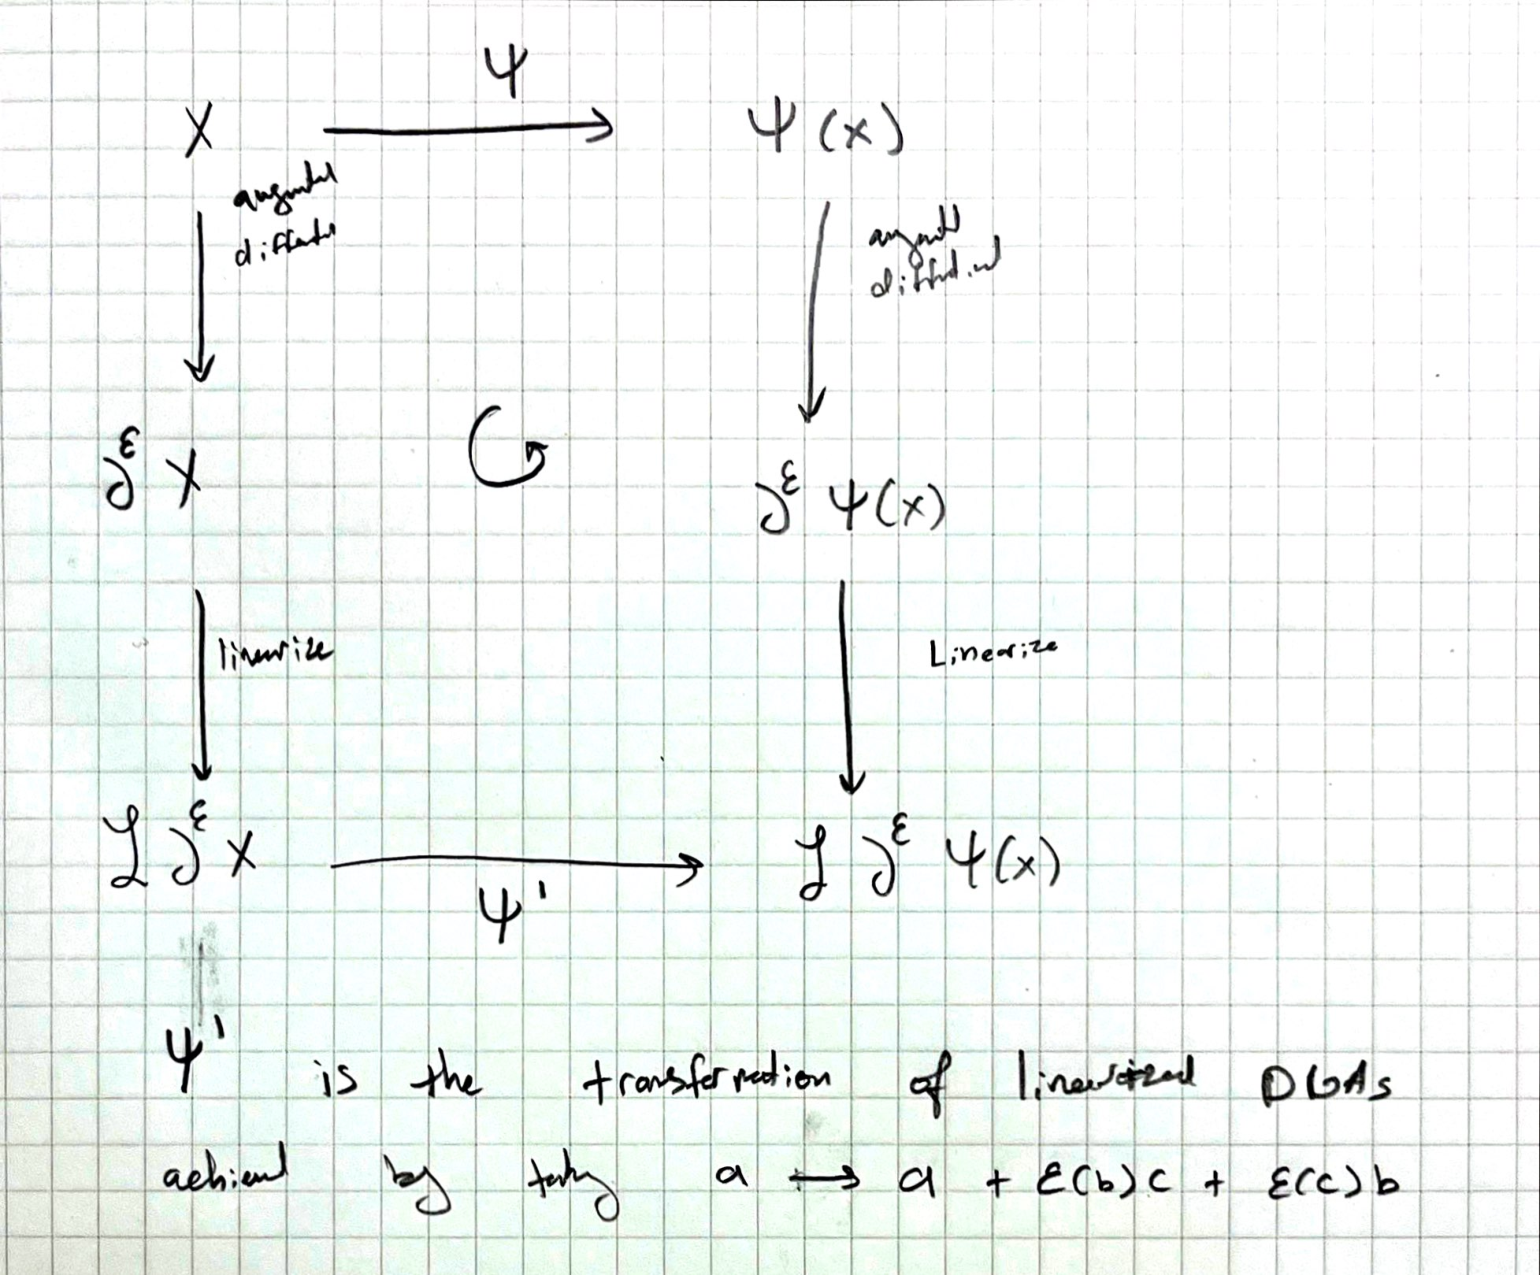
\includegraphics[width = 5in]{General-Information/Pictures/commutativediagram.pdf}

  
  
\end{figure}
















\end{proof}




\section{Questions?}

\subfile{General-Information/questions?.tex}

\section{Examples}

\subfile{General-Information/examples.tex}



\end{document}